\section{Saved-Data Details and Exploratory Associations}
\label{sec:saved-data-supplement}

The following analyses preserve their original populations, estimators and
uncertainty procedures. The exact readout table accompanies the main result.
Conditional candidate identities, same-cohort correctness associations and
in-sample concentration are exploratory or descriptive evidence. They do
not provide independent confirmation of expert usefulness. No outcome or
significance filter was applied to the saved correlation figure.

\subsection{Exact present-class readout estimates}

\begin{table}[t]
\centering\small
\begin{tabular}{lrrr}
\toprule
Model & Sentences & Loss change & Simultaneous 95\% CI \\
\midrule
GPT-OSS & 37,549 & $-0.07858$ & $[-0.09567,-0.06179]$ \\
Nemotron & 35,334 & $-0.13721$ & $[-0.15628,-0.11819]$ \\
Qwen3.5 & 34,740 & $-0.14090$ & $[-0.15359,-0.12781]$ \\
Qwen3.6 & 35,484 & $-0.13899$ & $[-0.15276,-0.12601]$ \\
Gemma & 31,902 & $-0.14866$ & $[-0.16136,-0.13692]$ \\
GLM & 38,931 & $-0.13679$ & $[-0.15302,-0.12035]$ \\
Qwen3-30B & 36,445 & $-0.09427$ & $[-0.10929,-0.08100]$ \\
\bottomrule
\end{tabular}
\caption{Routing-augmented minus retrospective judge-context
cross-entropy in the saved CLEAN readout. Each row has 522 questions and
509 families. Intervals retain the model-specific saved seven-comparison
procedure; this is not a fresh joint test across models. Sentences are
measurements within questions.}
\label{tab:analysis-readout}
\end{table}

\subsection{Selection frequency, motion and candidate experts}
For a window $W$, selection frequency is
\begin{equation}
f_{\ell,e}(W)=\frac{1}{|W|}\sum_{t\in W}
             \mathbf{1}\{e\in S_{\ell,t}\}.
\end{equation}
It sums to $k_\ell$, rather than one. Entropy or divergence of the mean
selection distribution therefore uses $f_{\ell,e}/k_\ell$.
If normalized executed weights are captured, their occupancy is a
different statistic; IDs alone cannot recover it.

Temporal continuity can be measured by
$|S_{\ell,t}\cap S_{\ell,t-d}|/k_\ell$ at declared lag $d$. A temporal claim
requires comparison with an order-shuffled control that preserves the
same allocation composition. Entropy of mean allocation minus mean
per-token entropy is invariant to token ordering and cannot establish a
state transition. Formulas, units, lag, support and required captured
fields belong beside every reported metric.

Conditional expert association is estimated within comparable source
conditions before averaging across problem families. A preserved
Qwen3.6 analysis nominates layer 28 experts 189 and 9: matched
selection-membership differences before a next-sentence Verify label are
$+0.08118$ and $+0.06296$, positive in 40/48 and 44/48 discovery families.
The analysis has 483 matched positive windows across 48 families, and
fold-selected proposals retain positive held-out directions. This is
conditional nomination under an LLM-assigned target; it does not make
these experts semantic modules or independently validate the final fixed
pair.

A candidate's rank is also estimator-dependent. In the legacy selector
audit, replacing accuracy-lift ranking with activation-rate differences
retains only 14/48 Qwen targets, 6/16 GPT positive targets and 7/16 GPT
negative targets under the same budgets. Analyses should report that
sensitivity, support and held-out stability. A low-frequency expert is
not thereby dispensable, and an expert correlated with an error is not
thereby harmful: difficult questions can cause both expert use and errors.

\subsection{Adjusted expert-profile associations with correctness}
\label{sec:adjusted-expert-associations}

The saved A-corpus analysis also relates whole-reasoning use of
class-enriched expert sets to adjudicated answer correctness. For each
class, the archived rule nominates up to three enriched experts per
selected layer from the full A corpus without using correctness labels.
The feature is their selected-slot count over all reasoning tokens,
divided by native $k$ and reasoning-token count, then averaged equally
across layers with a nominated set. It is not restricted to tokens
labelled with the nominating class, and different class sets can overlap.

Figure~\ref{fig:adjusted-expert-associations} presents all 49 model--class
cells. Each is a saved partial Pearson correlation after the original
adjustment for benchmark, log completion length, retrospective problem
difficulty, the class's share of labelled tokens and a cap indicator when
present. The difficulty estimate uses the other 31 same-model attempts
for AIME/AMC and the other six models on single-attempt datasets. It is a
retrospective analysis covariate, not an available deployment feature.
Question support ranges from 1,545 to 1,547 per model.

\begin{figure}[t]
\centering
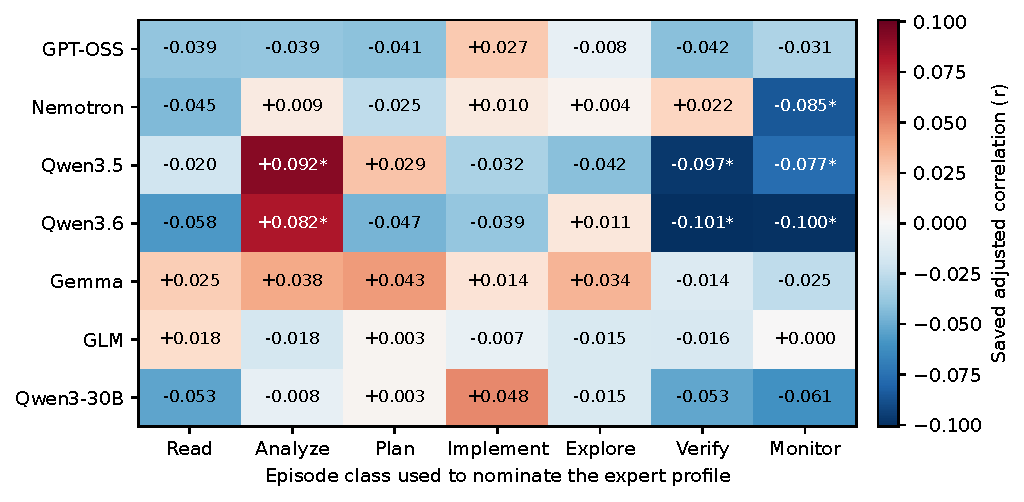
\includegraphics[width=\linewidth]{generated/model_analysis_review/expert_usage_correctness.pdf}
\caption{Saved nuisance-adjusted correlations between whole-reasoning use
of a class-nominated expert set and adjudicated correctness. All seven
models and seven classes are shown. Asterisks preserve the original
$q<0.05$ threshold from Benjamini--Hochberg correction within each model's
21 mean-feature comparisons (seven classes by all/in/out usage); they do
not represent a new joint test across the 49 displayed cells. Correlations
use the original same-cohort nomination and adjustment rules.}
\label{fig:adjusted-expert-associations}
\end{figure}

The largest corrected associations occur for Qwen3.5 and Qwen3.6:
Analyze-profile use correlates positively with correctness
($r=0.0918$ and $0.0818$), while Verify-profile use correlates negatively
($r=-0.0972$ and $-0.1008$), as does Monitor-profile use
($r=-0.0770$ and $-0.0995$). Nemotron's Monitor-profile association is
also below zero ($r=-0.0853$) at its original corrected threshold. The
remaining cells, including all cells for GPT-OSS, Gemma, GLM and
Qwen3-30B, do not pass that threshold. Differences in threshold crossings
are not tests of model differences.

The preserved confidence intervals use 1,000 question-ID bootstrap draws,
refitting nuisance regressions while holding the nominated sets and
difficulty estimates fixed. They do not cluster duplicate problem
families. Those intervals, support and all original $q$ values remain in
the accompanying source CSV. This is an exploratory association screen on
the nomination cohort. It supplies neither held-out expert usefulness nor
the effect of removing a Verify- or Monitor-associated expert.

\subsection{Labelled-state coverage under frequency-based retention}
\label{sec:labelled-coverage}

The saved seven-model A summaries allow a descriptive retention analysis
without another model run. Let $n_{\ell,e,c}$ count original selected
expert slots associated with labelled state $c$. For each layer, rank
experts by $\sum_c n_{\ell,e,c}$, breaking ties by expert ID, and retain
the first $b$ identities as $K_\ell(b)$. The state-specific coverage is
\begin{equation}
R_c(b)=\frac{\sum_\ell\sum_{e\in K_\ell(b)}n_{\ell,e,c}}
                  {\sum_\ell\sum_e n_{\ell,e,c}}.
\end{equation}
The pooled curve uses all seven classes in numerator and denominator;
the least-covered curve takes $\min_c R_c(b)$. Counts are weighted by
original token-layer selections, without equal-family or equal-benchmark
reweighting. The source A cohort contains 1,547 questions per model, but
labels cover only a subset of their reasoning tokens.

\begin{figure}[t]
\centering
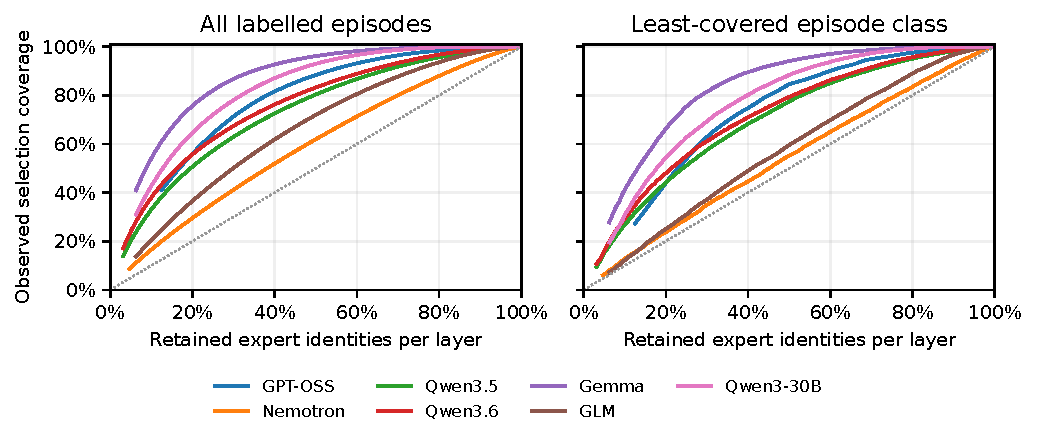
\includegraphics[width=\linewidth]{generated/model_analysis_review/labelled_expert_coverage.pdf}
\caption{In-sample coverage of original labelled expert selections when
retaining the most frequently selected identities within each layer.
Left: pooled labelled selections. Right: the least-covered episode class
at each retained count. The dotted line is the retained identity fraction,
not an evaluated random policy. The rank and coverage use the same data;
no model is pruned or rerun. Native selection coverage measures neither
accuracy nor memory saved.}
\label{fig:labelled-expert-coverage}
\end{figure}

Concentration differs substantially across these captured corpora
(Figure~\ref{fig:labelled-expert-coverage}). At the common plotting landmark
of half the expert identities per layer, pooled coverage is 88.34\% for
GPT-OSS, 61.90\% for Nemotron, 80.32\% for Qwen3.5, 83.20\% for Qwen3.6,
96.11\% for Gemma, 71.92\% for GLM and 92.94\% for Qwen3-30B. The
least-covered class retains respectively 84.58\%, 55.13\%, 77.39\%,
79.30\%, 94.04\%, 59.52\% and 88.35\%. Monitor is least covered in six
models; Read is least covered for Gemma. A pooled-frequency summary can
therefore conceal a larger coverage loss for a particular labelled state.

Half retention is a plotting landmark, not a selected deployment budget.
These deterministic summaries have no held-out stability estimate or
inferential interval. Their model differences also reflect generated text
and annotation coverage. They measure selected slots on native labelled
traces, not complete top-$k$ containment, executed-weight mass or coverage
of unlabelled tokens. The keep-sets have not been checked for grouped-router
feasibility. Changing a route can alter every subsequent token, so these
curves nominate analysis questions rather than predict post-pruning
accuracy or resident memory.


\subsection{Observed adjacent-state transitions}
\label{sec:saved-transitions}

The consecutive-sentence analysis also now covers all seven models on the
common 522-question/509-family population
(Figure~\ref{fig:expert-memory-transitions}). An edge requires consecutive
original sentence indices in the same reasoning segment; gaps and missing
labels break adjacency. Labelled-sentence coverage ranges from 7.0\% for
Qwen3.6 to 28.1\% for GPT-OSS. The matrices therefore describe observed labelled
adjacencies rather than complete reasoning trajectories. Cell/source family
support, coverage denominators and endpoint-censored dwell durations accompany
the saved transition receipt.

\begin{figure}[t]
\centering
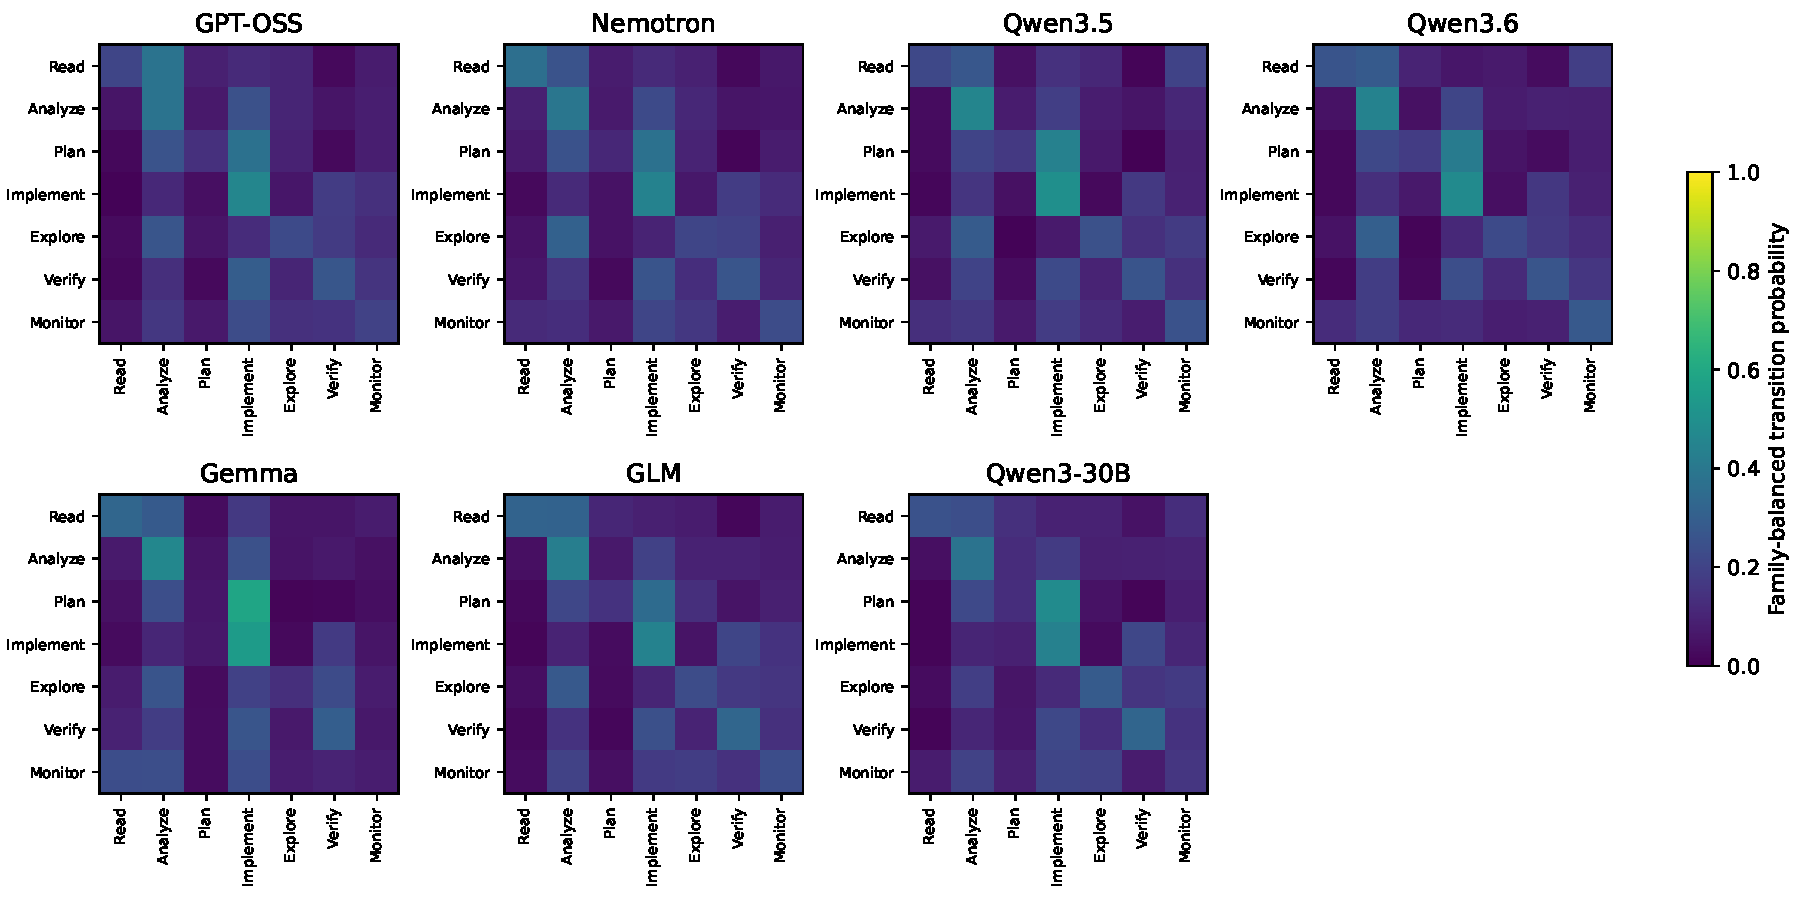
\includegraphics[width=\linewidth]{figures/expert_memory_transitions_r2.pdf}
\caption{Family-balanced next-class probabilities for consecutive observed
sentences, using the common 509-family population. Rows are current classes
and columns are next classes. Missing labels and sentence gaps break adjacency;
unsupported rows are missing.}
\label{fig:expert-memory-transitions}
\end{figure}


\subsection{Reproducible main-result figures}
The main-result figures are regenerated from three compact saved CSVs in
\texttt{generated/best\_results\_20261009/}. The bundle includes all seven
readout rows, all 105 model/fold/arm selection cells and the complete saved
anticipation export, including endpoints not promoted in the main text.
A standalone plotting script and SHA-256 manifests bind the inputs and
outputs. Confidence limits are copied unchanged; fold differences are
computed by pairing the original common folds, without new resampling or
scientific refitting. Historical uncertain and harmful intervention
outcomes remain in their respective appendices.
